\documentclass[10pt, aspectratio=149]{beamer}

% Language setting
% Replace `english' with e.g. `spanish' to change the document language
\usepackage[english]{babel}

\mode<presentation>{
\usetheme{Madrid}
\setbeamercovered{transparent}
\setbeamertemplate{navigation symbols}{}
}

% Useful packages
\usepackage{amsmath}
\usepackage{booktabs}
\usepackage{graphicx}
\usepackage{tabularx}
\usepackage{multicol}

\title[DistilBERT for Text Classification]{DistilBERT: An Effectively Complexity-reduced \\ Language Model for Text Classification}
% \subtitle{Final Project in Scientific Research Methodology (MNC)}
% \logo{
\includegraphics[scale=.3]{img/fithcmuslogo.png}}
\author[PNTAn and THQuan]{Pham Ngoc Thien An \inst{1,}\inst{2} and Tran Hoang Quan \inst{1,}\inst{2}}
\institute[fit@hcmus]{
\footnotemark[1]{Faculty of Information Technology, University of Science},

\footnotemark[2]{Vietnam National University, Ho Chi Minh City, Vietnam}
}
\date{June 01, 2023}
\begin{document}
\maketitle

\begin{frame}{Table of Contents}
\tableofcontents
\end{frame}

\section{Introduction}
\begin{frame}{Introduction}
\framesubtitle{Text Classification}
\begin{itemize}
\item Text Classification is the process of categorizing text documents into predefined classes based on their content
\item Its applications: document organization, news filtering, spam detection, opinion mining, and computational phenotyping
\end{itemize}

\begin{figure}
\centering
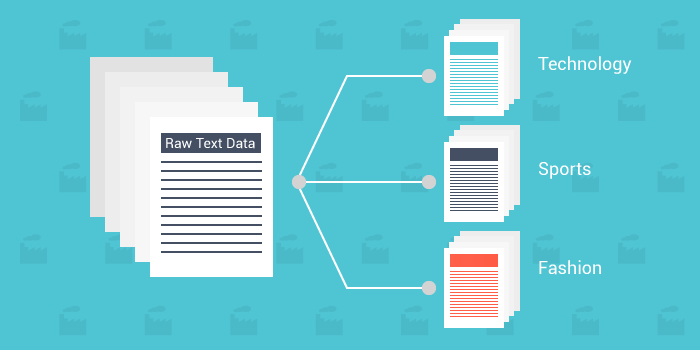
\includegraphics[width=80mm,scale=0.7]{img/TC_example.png}
\caption{Example of Text Classification}
\label{fig:example}
\end{figure}
\end{frame}

\begin{frame}{Introduction}
\framesubtitle{Observation and Motivation}
Observation:
\begin{itemize}
\item The depth necessitates a large number of parameters that must be loaded into memory, limiting to the training phase and may pose challenges in real-world scenarios (inference under low-latency constraints or fine-tuning with limited resources.)
\end{itemize}

Motivation: 
\begin{itemize}
\item Creating more compact models with fewer parameters (such as knowledge distillation based models)
\end{itemize}
\end{frame}

\begin{frame}{Introduction}
\framesubtitle{Contribution}
\begin{itemize}
\item Our proposal can be more appropriate for real-world appliances by its viability of inferencing under low-latency constraints or well-functioning in limited computational resources.
\item Our experimental results demonstrate that the proposal achieves comparable performance to SOTA text classification methods on several benchmark datasets.
\end{itemize}
    
\end{frame}
\section{Related Works}
\begin{frame}{Related Works}
sede vacante
\end{frame}
\section{Proposed Method}
\begin{frame}{Proposed Method}
\begin{columns}
\begin{column}{.5\textwidth}
\begin{itemize}
\item Sanh et al. (2019)\cite{Sanh2019} proposed DistilBERT as a smaller, faster, cheaper, lighter and distiled version of BERT.
\item By fine-tuning DistilBERT, we proposed a efficient model for Text Classfication.
\item The outputs of DistilBERT at token \texttt{[CLS]} is fed into a fully-connected layer with parameters $W \in \mathbb{R}^{D\times H}$ and $b \in \mathbb{R}^H$. In that, $D$ is the dimensionality of the output vector and H denotes the number of classes. Finally, to predict the label, the softmax layer is applied.
\end{itemize}

\end{column}

\begin{column}{.5\textwidth}
\begin{figure}[htp]
\centering
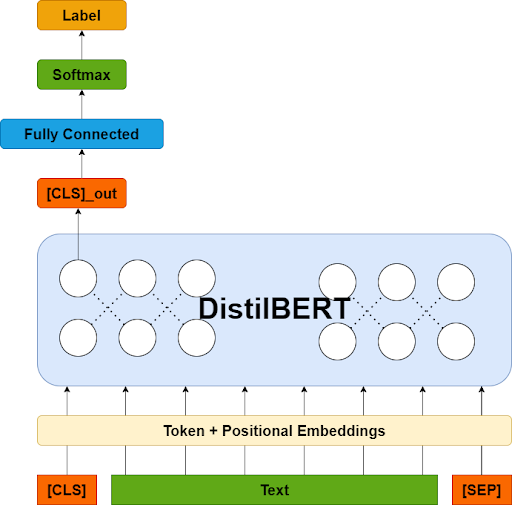
\includegraphics[scale=.3]{img/distilbert.png}
\caption{The overall architecture of our proposed method using DistilBERT.}
% \label{fig:distilbert}
\end{figure}
\end{column}
\end{columns}
\end{frame}
\section{Experiments}
\begin{frame}{Experiments and Results}
\framesubtitle{Baselines}
We compare our proposed method to several approaches, including
\begin{itemize}
\item Shallow approaches:
\begin{itemize}
\item Logistic Regression
\item Na\"ive Bayes
\item SVM
\end{itemize}
\item Deep approaches:
\begin{itemize}
\item BiGRU Sequence-to-Sequence
\item CNN and Multi-channel CNN with LSTM / BiGRU
\item Finetuned LLMs: BERT and finetuned XLM-RoBERTa.
\end{itemize}
\end{itemize}
\end{frame}

\begin{frame}{Experiments (cont.)}
\framesubtitle{Datasets}

We conduct experiments on two datasets TREC (multiclass) and SST2 (binary class).

\begin{table}
\centering
\begin{tabular}{|c|c|c|}\hline%c|c|c|} \hline
\textbf{Training} & \textbf{Testing} & \textbf{Coarse labels} \\ \hline%& \textbf{Fine class labels} & \textbf{Avg. length} & \textbf{Vocab. size} \\ \hline
5500              & 500              & 6                    \\ \hline %  & 50                         & 10                   & 8700                 \\ \hline
\end{tabular}
\caption{Statistics of the TREC dataset} \label{tab:trec-insight}
\end{table}

\begin{table}
\centering
\begin{tabular}{|c|c|c|c|} \hline
\textbf{Training} & \textbf{Validation} & \textbf{Testing} & \textbf{Labels} \\ \hline
47144              & 20205              & 872                      & 2 \\ \hline
\end{tabular}
\caption{Statistics of the SST2 dataset} \label{tab:sst2-insight}
\end{table}
\end{frame}

\begin{frame}{Experiments (cont.)}
\framesubtitle{Metrics}

We use Accuracy, Precision, Recall and F1 score as evaluation metrics.
\begin{equation}
Accuracy  = \displaystyle\frac{1}{n}\sum_{i = 1}^n (y_i = \hat{y_i})
\end{equation}

With $TP, FP$ and $FN$ are True Positives, False Positives and False Negatives samples, respectively:

\begin{equation}
\begin{aligned}
Precision\ (P) &= \frac{TP}{TP + FP} \\
Recall\ (R) &= \frac{TP}{TP + FN} \\
F_{1} &= \frac{2PR}{P + R}    
\end{aligned}
\end{equation}
\end{frame}

\begin{frame}{Experiments (cont.)}
\framesubtitle{Setup}
\end{frame}

\begin{frame}{Results}
\framesubtitle{Performance Analysis - TREC dataset}

\begin{table}
\small{
\begin{tabular*}{\linewidth}{@{\extracolsep\fill}lcccc}
\hline
\textbf{Model}                & \textbf{Accuracy} & \textbf{Precision} & \textbf{Recall} &  \textbf{F1} \\ \hline
Logistic Regression   & 0.852 & 0.831          & 0.897       & 0.856  \\ 
Multinomial Naive Bayes   & 0.832 & 0.704          & 0.699       & 0.697 \\ 
Support Vector Classifier & 0.886 & 0.862          & 0.912       & 0.882  \\ \hline
BiGRU Seq2Seq            & 0.836 & 0.695          & 0.708       & 0.700  \\ \hline
CNN + random embedding                 & 0.726 & 0.809          & 0.684       & 0.718   \\
CNN + fastText (freeze)   & 0.924 & 0.933          & 0.898       & 0.912    \\
CNN + fastText (trainable) & 0.910 & 0.922          & 0.885       & 0.899    \\ \hline
CNN + LSTM + random embedding  & 0.652 & 0.717          & 0.637       & 0.631  \\
CNN + BiGRU + random embedding     & 0.676 & 0.717          & 0.701       & 0.689   \\
CNN + BiGRU + fastText (freeze)   & 0.914 & 0.919          & 0.896       & 0.904  \\
CNN + BiGRU + fastText (trainable) & 0.902 & 0.892          & 0.884       & 0.886 \\ \hline
Finetuned BERT & \textbf{0.976} & \textbf{0.978} & \textbf{0.982} & \textbf{0.979}  \\
Finetuned XLM-RoBERTa & 0.966 & 0.971          & 0.970       & 0.970  \\ \hline
Finetuned DistilBERT  & 0.974 & 0.976 & 0.977  & 0.976  \\ \hline
\end{tabular*}
}
\caption{Experiment metrics on the TREC dataset. Bold indicates the highest scores.} \label{tab:result-TREC}
\end{table}
\end{frame}

\begin{frame}{Results (cont.)}
\framesubtitle{Performance Analysis - SST2 dataset}
\begin{table}
\small{
\begin{tabular*}{\textwidth}{@{\extracolsep\fill}lcccc}
\hline
\textbf{Model}                & \textbf{Accuracy} & \textbf{Precision} & \textbf{Recall} &  \textbf{F1} \\ \hline
Logistic Regression   & 0.807 & 0.806 & 0.810 & 0.807 \\ 
Multinomial Naive Bayes   & 0.808 & 0.807 & 0.819 & 0.806 \\ 
Support Vector Classifier & 0.829 & 0.829 & 0.830 & 0.829  \\ \hline
BiGRU Seq2Seq  & 0.765 & 0.766 & 0.764 & 0.764 \\ \hline
CNN + random embedding  & 0.760 & 0.774 & 0.758 & 0.756   \\
CNN + fastText (freeze)   & 0.830 & 0.834 & 0.829 & 0.830 \\
CNN + fastText (trainable) & 0.843 & 0.851 & 0.842 & 0.842 \\ \hline

CNN + LSTM + random embedding  & 0.734 & 0.741 & 0.735 & 0.733  \\
CNN + BiGRU + random embedding     & 0.748 & 0.754 & 0.749 & 0.747   \\
CNN + BiGRU + fastText (freeze)   & 0.815 & 0.818 & 0.816 & 0.815  \\
CNN + BiGRU + fastText (trainable) & 0.806 & 0.813 & 0.805 & 0.805 \\ \hline 
Finetuned BERT & 0.906 & 0.905 & 0.909 & 0.906  \\
Finetuned XLM-RoBERTa & \textbf{0.911} & \textbf{0.911} & \textbf{0.911} & \textbf{0.911}  \\ \hline
Finetuned DistilBERT  & 0.905 & 0.904 & 0.906 & 0.905  \\ \hline
\end{tabular*}
}
\caption{Experiment metrics on the SST2 dataset. Bold indicates the highest scores.} \label{tab:result-SST2}
\end{table}
\end{frame}

\begin{frame}{Results (cont.)}
\framesubtitle{Inference Time Analysis}

\begin{table}
\small{
\begin{tabular*}{\textwidth}{@{\extracolsep\fill}lccc}
\toprule
 & \multicolumn{2}{@{}c@{}}{\textbf{Inference time}} \\ \cmidrule{2-3}%
\textbf{Model}  & \textbf{TREC}  & \textbf{SST2}\\ \toprule
BiGRU Seq2Seq                      & 1.812 $\pm$ 0.668 ms &  3.394 $\pm$ 1.222 ms                     \\ \midrule
CNN + random embedding             & 1.673 $\pm$ 0.359 ms & 2.378 $\pm$ 0.747 ms                  \\
CNN + fastText (freeze)           & 1.610 $\pm$ 0.318 ms & 1.705 $\pm$ 0.379 ms                     \\
CNN + fastText (trainable)         & 1.658 $\pm$ 0.444 ms & 1.780 $\pm$ 0.329 ms                    \\ \midrule
CNN + LSTM + random embedding      & 5.626 $\pm$ 0.750 ms & 6.607 $\pm$ 1.010 ms                   \\
CNN + BiGRU + random embedding     & 11.387 $\pm$ 3.077 ms & 10.419 $\pm$ 1.635 ms                   \\
CNN + BiGRU + fastText (freeze)   & 10.211 $\pm$ 1.460 ms & 11.769 $\pm$ 3.032 ms                  \\
CNN + BiGRU + fastText (trainable) & 10.270 $\pm$ 2.187 ms & 13.386 $\pm$ 3.206 ms                  \\ \midrule
Finetuned BERT                     & 17.725 $\pm$ 4.071 ms & 16.984 $\pm$ 4.228 ms                  \\
Finetuned XLM-RoBERTa              & 16.933 $\pm$ 8.987 ms & 15.848 $\pm$ 3.840 ms                  \\ \midrule
Finetuned DistilBERT               & 9.776 $\pm$ 2.499 ms & 9.629 $\pm$ 6.478 ms                    \\ \bottomrule
\end{tabular*}
}
\caption{Inference time of deep learning approaches on testing sets}\label{tab:inference-result}
\end{table}
\end{frame}

\begin{frame}{Results (cont.)}
\framesubtitle{Parameter Analysis}
\begin{table}
\small{
\begin{tabular*}{\textwidth}{@{\extracolsep\fill}lccc}
\toprule
 & \multicolumn{2}{@{}c@{}}{\textbf{Total parameters}} \\ \cmidrule{2-3}%
\textbf{Model}  & \textbf{TREC}  & \textbf{SST2}\\ \midrule
BiGRU Seq2Seq                      & 18,461,702 &  20,254,722                     \\ \midrule
CNN + random embedding             & 3,192,606 & 4,802,702                  \\
CNN + fastText (freeze)           & 362,106 & 360,902                     \\
CNN + fastText (trainable)         & 3,192,606 & 4,802,702                    \\ \midrule
CNN + LSTM + random embedding      & 4,420,416 & 6,568,012                   \\
CNN + BiGRU + random embedding     & 4,504,896 & 6,652,492                   \\
CNN + BiGRU + fastText (freeze)   & 987,696 & 986,892                  \\
CNN + BiGRU + fastText (trainable) & 6,648,696 & 9,870,492                 \\ \midrule
Finetuned BERT                     & 108,314,886 & 108,311,810                  \\
Finetuned XLM-RoBERTa              & 278,048,262 & 278,045,186                  \\ \midrule
Finetuned DistilBERT  & 65,786,118 & 65,783,042                    \\ \bottomrule
\end{tabular*}
}
\caption{Total parameters of deep learning approaches}\label{tab:parameters-result}
\end{table}
\end{frame}
\section{Conclusion}
\begin{frame}{Conclusion} 
\begin{itemize}
\item In this work, we propose the method of using DistilBERT -- a cheaper, lighter, and faster version of BERT -- for Text Classification. Even though reducing the number of layers (e.g., attention heads), DistilBERT still shows its efficiency by the comparable achievements.
\item However, in this work, we only focus on investigating the architecture used without considering how to integrate more useful information (e.g., structural or hierarchical) to capture more meaningful contextual features. We leave this for future research.
\end{itemize}
\end{frame}

% Citation
\section{References}
\begin{frame}[allowframebreaks]{References}
\bibliographystyle{ieeetr}
\bibliography{cite/ref}
\end{frame}

\begin{frame}[plain]
\centering
\Huge{\textbf{Thanks for listening!}}

\small{\textbf{Q\&A}}
\end{frame}

\end{document}